\documentclass[
11pt, % Set the default font size, options include: 8pt, 9pt, 10pt, 11pt, 12pt, 14pt, 17pt, 20pt
%t, % Uncomment to vertically align all slide content to the top of the slide, rather than the default centered
%aspectratio=169, % Uncomment to set the aspect ratio to a 16:9 ratio which matches the aspect ratio of 1080p and 4K screens and projectors
]{beamer}

\graphicspath{{Images/}{./}} % Specifies where to look for included images (trailing slash required)

\usepackage{todonotes}
\usepackage{graphicx}
\usepackage{xcolor}
\usepackage{subfig}
%%\usepackage[noend]{algpseudocode}

%
%\usepackage{algorithm}
%\usepackage{algorithmic}
\usepackage{algorithm}
\usepackage{algpseudocode}
\usepackage{blkarray}
\usepackage{amsmath}
\usepackage{xspace}
\usepackage{float}


\usepackage{tikz}
\usetikzlibrary{matrix, decorations, patterns, positioning, shapes, calc, intersections, arrows, fit}

\usetikzlibrary{patterns}
\usetikzlibrary{fit,calc,positioning,decorations.pathreplacing,matrix,3d, hobby}

\usepackage{booktabs} % Allows the use of \toprule, \midrule and \bottomrule for better rules in tables
\usepackage{bm}
\usepackage{multirow}
\usepackage{ragged2e}


\newcommand{\brown}[1]{{\color{brown} #1 }}

%% Colors from https://latexcolor.com/
\definecolor{pastelviolet}{rgb}{0.8, 0.6, 0.79}
\definecolor{babyblueeyes}{rgb}{0.63, 0.79, 0.95}
\definecolor{pastelyellow}{rgb}{0.99, 0.99, 0.59}
\definecolor{pastelgreen}{rgb}{0.47, 0.87, 0.47}
\definecolor{pastelred}{rgb}{1.0, 0.41, 0.38}
\colorlet{patternblue}{blue!60}



%%\newcommand{\tensorcolor}{patternblue}
\newcommand{\tensorcolor}{cyan}


\colorlet{darkred}{red!80!black}
\colorlet{darkblue}{blue!80!black}
\newcommand<>{\darkred}[1]{{\color{darkred}{#1}}}
\newcommand<>{\darkblue}[1]{{\color#2{blue!50!black!100}{#1}}}

\newcommand{\A}{\mathbf{A}}
\newcommand{\B}{\mathbf{B}}
\newcommand{\CC}{\mathbf{C}}
%\newcommand{\Real}{\mathbb{R}}
%\newcommand{\vc}[1]{\bm{#1}}

\usetheme{Madrid}

%\newcommand{\Tra}{{\sf T}} 


%\newcommand{\Ms}[2]{\mathbf{#1}^{(#2)}} 
%\newcommand{\M}[1]{\mathbf{#1}} 
%\newcommand{\Mb}[2]{\mathbf{#1}_{#2}} 
%\newcommand{\Mbs}[3]{\mathbf{#1}_{#2}^{(#3)}} 

%\usepackage{enumitem}

\input{../tensor_header}

\hypersetup{linkcolor=blue}

%----------------------------------------------------------------------------------------
%	PRESENTATION INFORMATION
%----------------------------------------------------------------------------------------

\title[Multi-TTM]{Multiple Tensor Times Matrix computation} % The short title in the optional parameter appears at the bottom of every slide, the full title in the main parameter is only on the title page

%\subtitle{Optional Subtitle} % Presentation subtitle, remove this command if a subtitle isn't required

\author[Suraj Kumar]{Suraj Kumar} % Presenter name(s), the optional parameter can contain a shortened version to appear on the bottom of every slide, while the main parameter will appear on the title slide

\institute[Inria \& ENS Lyon]{Inria \& ENS Lyon \\ \smallskip Email:\textit{suraj.kumar@inria.fr}} % Your institution, the optional parameter can be used for the institution shorthand and will appear on the bottom of every slide after author names, while the required parameter is used on the title slide and can include your email address or additional information on separate lines

\date[CR12]{CR12: October 2023\\ \smallskip\small https://surakuma.github.io/courses/daamtc.html} % Presentation date or conference/meeting name, the optional parameter can contain a shortened version to appear on the bottom of every slide, while the required parameter value is output to the title slide

%----------------------------------------------------------------------------------------

\begin{document}
	
	%----------------------------------------------------------------------------------------
	%	TITLE SLIDE
	%----------------------------------------------------------------------------------------
	
	\begin{frame}
		\titlepage % Output the title slide, automatically created using the text entered in the PRESENTATION INFORMATION block above
	\end{frame}

\begin{frame}{Tucker decomposition of $\T{A} \in \mathbb{R}^{n_1\times n_2\times\cdots\times n_d}$}
	
	\small
	It represents a tensor with $d$ matrices (usually orthonormal) and a small core tensor.
	\vspace*{-0.25cm}\begin{center}
		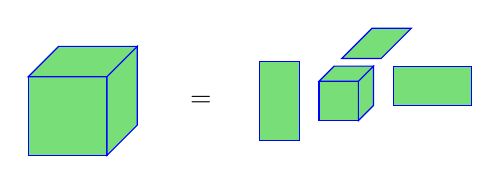
\begin{tikzpicture}[scale=0.25, every node/.style={transform shape}]
		\pgfmathsetmacro{\cubex}{4}
		\pgfmathsetmacro{\cubey}{4}
		\pgfmathsetmacro{\cubez}{4}
		\draw[blue,fill=pastelgreen] (-12,1,\cubez-2) -- ++(-\cubex,0,0) -- ++(0,-\cubey,0) -- ++(\cubex,0,0) -- cycle;
		\draw[blue,fill=pastelgreen] (-12,1,\cubez-2) -- ++(0,0,-\cubez) -- ++(0,-\cubey,0) -- ++(0,0,\cubez) -- cycle;
		\draw[blue,fill=pastelgreen] (-12,1,\cubez-2) -- ++(-\cubex,0,0) -- ++(0,0,-\cubez) -- ++(\cubex,0,0) -- cycle;
		\node[draw=none, text=black, scale=4] at (-8,-1,0) {$=$};
		
		\pgfmathsetmacro{\cubex}{2}
		\pgfmathsetmacro{\cubey}{2}
		\pgfmathsetmacro{\cubez}{2}
		\draw[blue,fill=pastelgreen] (0,0,0) -- ++(-\cubex,0,0) -- ++(0,-\cubey,0) -- ++(\cubex,0,0) -- cycle;
		\draw[blue,fill=pastelgreen] (0,0,0) -- ++(0,0,-\cubez) -- ++(0,-\cubey,0) -- ++(0,0,\cubez) -- cycle;
		\draw[blue,fill=pastelgreen] (0,0,0) -- ++(-\cubex,0,0) -- ++(0,0,-\cubez) -- ++(\cubex,0,0) -- cycle;
		
		\draw[blue,fill=pastelgreen] (-\cubex-1,1,0) -- ++(-\cubex,0,0) -- ++(0,-\cubey-2,0) -- ++(\cubex,0,0) -- cycle;
		\draw[blue,fill=pastelgreen] (\cubex+2+1,0,-\cubey) -- ++(-\cubex-2,0,0) -- ++(0,-\cubey,0) -- ++(\cubex+2,0,0) -- cycle;
		
		\draw[blue,fill=pastelgreen] (0,0,-\cubez-1) -- ++(-\cubex,0,0) -- ++(0,0,-\cubez-2) -- ++(\cubex,0,0) -- cycle;
		\end{tikzpicture}
	\end{center}
	\vspace*{-0.15cm}\centering{\footnotesize Tucker decomposition of a $3$-dimensional tensor.}
	\vfill
	{\footnotesize\vspace*{-0.1cm}$$\T{A} = \T{G} \times_1 U_1 \cdots \times_d U_d$$
		$$\T{A}(i_1,\cdots,i_d) = \sum_{\alpha_1=1}^{r_1}\cdots\sum_{\alpha_d=1}^{r_d} \T{G}(\alpha_1,\cdots,\alpha_d)U_1(i_1,\alpha_1)\cdots U_d(i_d, \alpha_d)$$}
	\vfill
	\justifying
	It can be concisely expressed as $\T{A} = \llbracket \T{G}; U_1, \cdots, U_d\rrbracket $.
	\vfill
	Here $r_j$ for $1\le j\le d$ denote a set of ranks. Matrices $U_j \in \mathbb{R}^{n_j\times r_j}$ for $1\le j \le d$ are usually orthonormal and known as factor matrices. The tensor $\T{G}\in \mathbb{R}^{r_1\times r_2\times\cdots\times r_d}$ is called the core tensor. 	
\end{frame}

\begin{frame}{\large High Order SVD (HOSVD) for computing a Tucker decomposition}
	\small
	\begin{algorithm}[H]{
			\caption{HOSVD method to compute a Tucker decomposition}
			\begin{algorithmic}[1]
				\Require input tensor $\T{A}\in \mathbb{R}^{n_1\times \cdots \times n_d}$, desired rank $(r_1,\cdots, r_d)$
				\Ensure  $\T{A} = \T{G} \times_1 U_1 \times_2 U_2  \cdots \times_d U_d$
				\For{$k=1 \text{ to } d$}
				\State $U_k \gets r_k$ leading left singular vectors of $A_{(k)}$
				\EndFor
				\State $\T{G} = \T{A} \times_1 U_1^\Tra \times_2 U_2^\Tra  \cdots \times_d U_d^\Tra$
			\end{algorithmic}
	}\end{algorithm}
	
	
	\vfill
	\begin{itemize}
		\item When $r_i < rank(A_{(i)})$ for one or more $i$, the decomposition is called the truncated-HOSVD (T-HOSVD)
		\vfill
		\item The collective operation $\T{A} \times_1 U_1^\Tra \times_2 U_2^\Tra  \cdots \times_d U_d^\Tra$ is known as Multiple Tensor-Times-Matrix (Multi-TTM) computation
	\end{itemize}
\end{frame}
\begin{frame}{\large Sequentially T-HOSVD (ST-HOSVD) for Tucker decomposition}
	\small
	\begin{itemize}
		\item This method is more work efficient than T-HOSVD
		\vfill
		\item In each step, it reduces the size of one dimension of the tensor
	\end{itemize}
	
	%	\small
	\vspace{-0.25cm}\begin{algorithm}[H]{
			\caption{ST-HOSVD method to compute a Tucker decomposition}
			\begin{algorithmic}[1]
				\Require input tensor $\T{A}\in \mathbb{R}^{n_1\times \cdots \times n_d}$, desired rank $(r_1,\cdots, r_d)$
				\Ensure  $\llbracket \T{G}; U_1, \cdots, U_d\rrbracket $ : a $(r_1, \cdots, r_d)$-rank Tucker decomposition of $\T{A}$
				\State $\T{B} \gets \T{A}$
				\For{$k=1 \text{ to } d$}
%				\State $S\gets B_{(k)}B_{(k)}^T$
				\State $U_k \gets r_k$ leading singular vectors of $B_{(k)}$
				\State $\T{B} \gets \T{B} \times_k U_k$
				\EndFor
				\State $\T{G} = \T{B}$
			\end{algorithmic}
	}\end{algorithm}
%\vspace{-0.215cm}
We can note that ST-HOSVD also performs Multi-TTM computation by doing a sequence of TTM operations, i.e, $\T{G} =((\T{A} \times_1 U_1)\times_2 U_2) \cdots \times_d U_d $.
\end{frame}

\begin{frame}{Bottleneck computations for algorithms to compute Tucker decompositions}
	\begin{itemize}
		\item Multi-TTM becomes the overwhelming bottleneck computation when
		\begin{itemize}
			\item Matrix SVD costs are reduced using randomization via sketching or
			\item $U_k$ are computed with eigen value decompositions of $B_{(k)}B_{(k)}^T$
		\end{itemize}  --  
	\end{itemize}
\end{frame}
%\begin{frame}{}
%	content...
%\end{frame}



\section{CP decomposition}
	\begin{frame}{Table of Contents}		
		\tableofcontents[currentsection,hideallsubsections] % Output the table of contents (all sections on one slide)		
	\end{frame}

\end{document} 